\section{Attitude Determination and Control Subsystem}
\subsection{Location and Attitude Determination}
\subsubsection{Global Positioning System}
The SnapSat uses a GPS to determine its latitudinal and longitudinal position above the surface of the earth.  An Adafruit Ultimate GPS Breakout Version 3 which has an attitudinal limit of 40km was selected for the balloon launch.  As this GPS only has a rating up to 40km it will not be suitable for a space mission.  
\subsubsection{Inertial Measurement Unit}
The inertial measurement unit (IMU) that was selected for the balloon launch is a 10 degree of freedom (DOF) Adafruit IMU.  It includes a 3DOF magnetometer, a 3D0F accelerometer and a 3DOF gyroscope as well as a barometric pressure/altitude sensor which also includes temperature.  The IMU uses an Attidude Heading and Reference System (AHRS) algorithm that returns the pitch, yaw and roll of the satellite with respect to magnetic north.  Given the fact that this is a very cheap IMU there is a degree of drift associated with the gyroscope which causes inaccuracies.  There is also an error associated with the accelerometer however it is less than the the drift caused by the gyroscope. As such the accelerometer has been used to determine the attitude both for the balloon launch and in the functional testing as the photodiode system will not be functional in either of these tests.\\
In terms of the application in space for this component, the major problem with this IMU is that it is not radiation hardened which will result in larger errors the longer it remains in orbit and will eventually cause it to stop working.  Thus in the event of an actual space launch, this component would need to be replaced with a radiation and preferably more accurate component.  The other major error that effects the IMU is accumulated error which is directly related to the amount of time spent in orbit.  Although this may be reduced in higher quality IMU's it will always be an issue.  Thus a secondary orientation system is required in order to determine the attitude of the SnapSat accurately.
\subsubsection{Photodiode Sun Sensor System}
A photodiode based sun sensor system was selected to be the secondary orientation system in order to recalibrate the IMU and to use in long duration missions.  This system was primarily selected because it provides enough pointing accuracy for the purposes of this mission and is significantly cheaper than the alternatives of star trackers or actual sun sensors.  The actual component that was selected is an OSRAM SFH203P Photodiode.  Although these are simply off the shelf components, a cover glass can be placed over the photodiodes in order to protect them from UV radiation.\\
There are two common methods for placing photodiodes on a cubesat.  The first is to use six photodiodes that are orthogonal, one for each side. However this method does not provide photodiode coverage sufficient for sun vector estimation over the entire attitude sphere because the field of view of individual photodiodes is generally less than 180\textdegree.  The second method is to place pairs of photodiodes angled in a single plane which allows the sun vector component in the common plane to be measured as shown in the figure below:\\
\vspace{-6mm}
\begin{center}
    \begin{figure}[H]
        \caption{Sun Vector in a Plane \cite{Photo}}
        \vspace{-4mm}
        \centering
        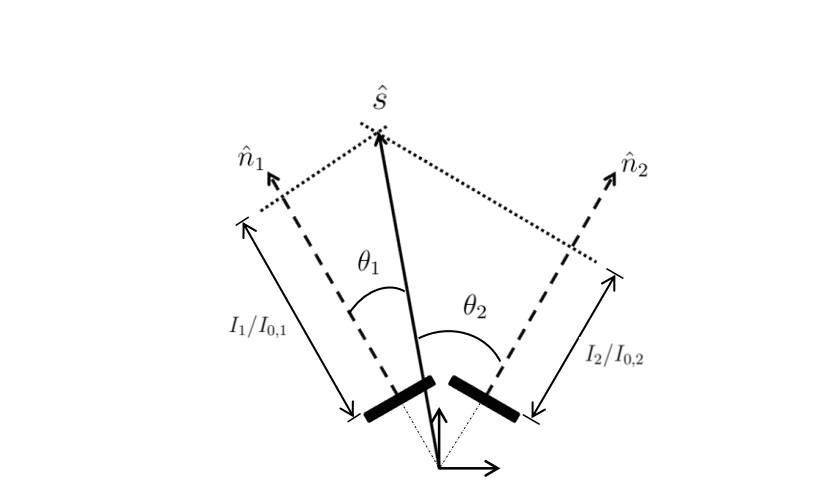
\includegraphics[scale = 0.4]{./figures/Sun_Vector}
    \end{figure}
\end{center}
\vspace{-5mm}
The three axis vector is then formulated by finding the intersection of multiple planes. For the space launch of SnapSat, the second method will be utilised in order to enable attitude calculation throughout the entire attitude sphere during orbit. Photodiodes output current as a function of the light intensity and angle to the light source. Thus utilising the information from the photodiodes a three dimensional sun vector can be created using the following equation \cite{Springmann}:
The photodiode system has limitations caused by occlusion, which is when the sensor's view of the Sun is blocked and albedo, which is when reflected sunlight from the earth or the moon distorts the reading. \cite{Leake}
\subsection{Attitude Control System}
\subsubsection{Selection of Magnetorquers}
The SnapSat is a 1kg cubesat with low mass, power and budget considerations. Subsequently, given these constraints, it was determined that magnetorquers would be the simplest and most cost efficient way to control the satellite.  To determine a rough estimate for the system requirements and available options, the magnetorquers for a number of similar cubesats were compared, as can be seen in the table below:\\
\vspace{-6mm}
\begin{center}
    \begin{figure}[H]
        \caption{Comparison of Control Systems for Current Satellites \cite{Miller}}
        \vspace{-4mm}
        \centering
        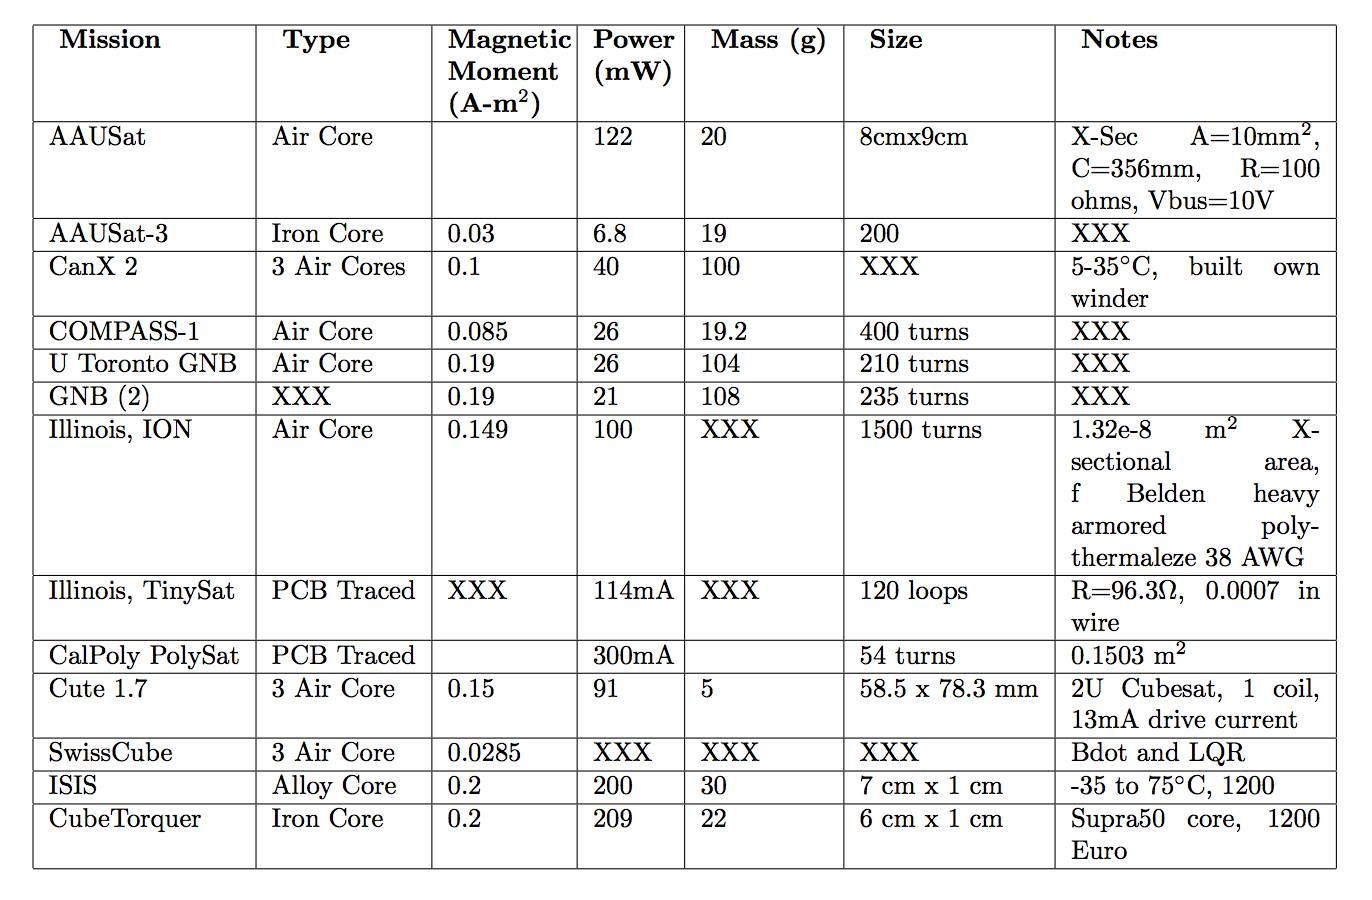
\includegraphics[scale = 0.4]{./figures/Magnetic_Moment}
    \end{figure}
\end{center}
\vspace{-5mm}
Using the comparison with the control systems for current satellites, it was determined that the SnapSat would require magnetorquers of approximately 0.1 to 0.15$Am^2$.  Due to the need to be designed and built in house an air core magnetorquer was selected rather than iron or alloy core.  To control the satellite attitude in all three axis, the SnapSat will require three seperate magnetorquers, one for each axis.  To further reduce power requirements the attitude control system will be set up so that only two of the magnetorquers can be turned on at any one time.  This will allow each individual magnetorquer to use more power and as such draw a higher current than would otherwise have been the case. 
\subsubsection{Design of Magnetorquer}
The torque on the satellite produced by the magnetorquer is given by cross product of the magnetic dipole of the magnetorquer and the earths magnetic field strength: 
\begin{center}
    $T = M \times B$
\end{center}
It is impossible to change the earth's magnetic field strength which is approximately $3 \times 10^{-6}$ Tesla.  Thus in order to maximise the torque on the satellite the magnetic dipole must be maximised. The magnetic dipole for the magnetorquer is given by the following equation:
\begin{center}
    $M = N \cdot I \cdot A$
\end{center}
Thus the magnetic dipole is dependent on the number of turns in the coil, the current through the wire and the area of the coil.  Initially it seems like a simple problem where the dipole will simply increase with the number of turns if the current and area are held constant.  However, this view does not take into account the resistance that increases with the length of wire, which given the fixed voltage will limit the current.  Due to cost restrictions, only 0.18mm round copper wire was available for use, which had a resistance per metre ($R_m$) of 0.646 ohms.  The following equations were then combined with the magnetic dipole equation in order to optimise the number of turns required:
\begin{center}
    $I = \frac{V}{R}$\vspace{2mm}\\
    $R = N \cdot Perimeter \cdot R_m$ \vspace{2mm}\\
    $P = V \cdot I$
\end{center}
When combined the following equation was determined:
\begin{center}
    $1 = \frac{4 \cdot M \cdot R_m}{V \cdot A}$
\end{center}
Thus since resistance per metre and voltage are constant, and perimeter is dependent on area, the magnetic dipole becomes constant for a given area.  Due to the restrictions in the lab only two sizes were available for the magnetorquers. The larger size was selected with side lengths of 0.073m as when the smaller size was modelled, the current draw was too high causing a higher level of power to be used.  Thus given this fixed area, the maximum magnetic dipole was determined to be  0.14$Am^2$.  Using this maximum dipole as the basis, the other characteristics of the magnetorquer were determined and can be viewed in the table below.
\begin{table}[H]
    \begin{center}
        \caption{Predicted Data for the Magnetorquers}
        \begin{tabular}{|c|c|c|c|c|c|c|c|}
            \hline
            Magnetic Dipole & Number of Turns & Current & Area & Voltage & Resistance & Power Required\\
            \hline
            0.14$Am^2$ & 132 & 0.2A & 0.005329$m^2$ & 5V & 24.9$\Omega$ & 1W\\
            \hline
        \end{tabular}
    \end{center}
    \vspace{-6mm}
\end{table}
\subsubsection{Construction of Magnetorquers}
As mentioned previously the Magnetorquers were built in house using equipment provided in the space lab.  The following procedure was applied to make each magnetorquer:
\begin{enumerate}
    \item The metal structural mould for the magnetorquer was unscrewed and sticky tape was applied to areas that were likely to come into contact with glue.
    \item The mould was placed in the winder and the copper wire was set up as shown in the photographs below.
    \begin{center}
        \begin{figure}[H]
            \caption{Magnetorquer Construction Set Up}
            \begin{subfigure}{0.5\textwidth}
                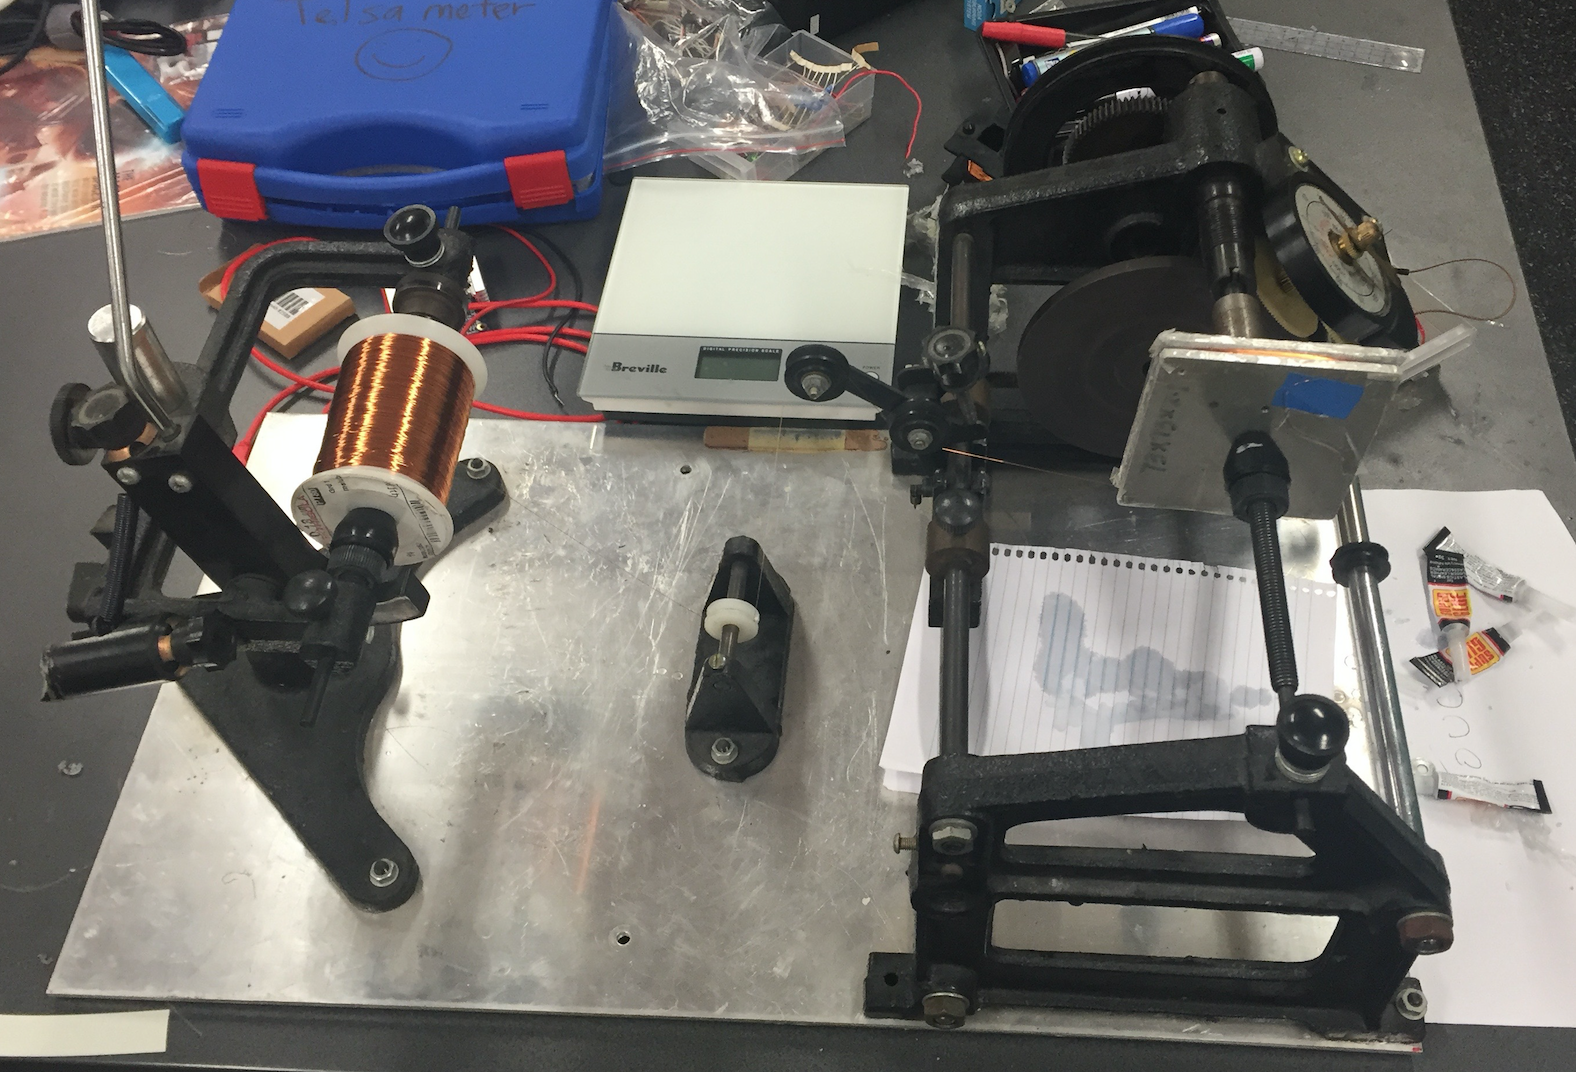
\includegraphics[scale = 0.35]{./figures/Construction_1}
            \end{subfigure}
            \hspace{15mm}
            \begin{subfigure}{0.5\textwidth}
                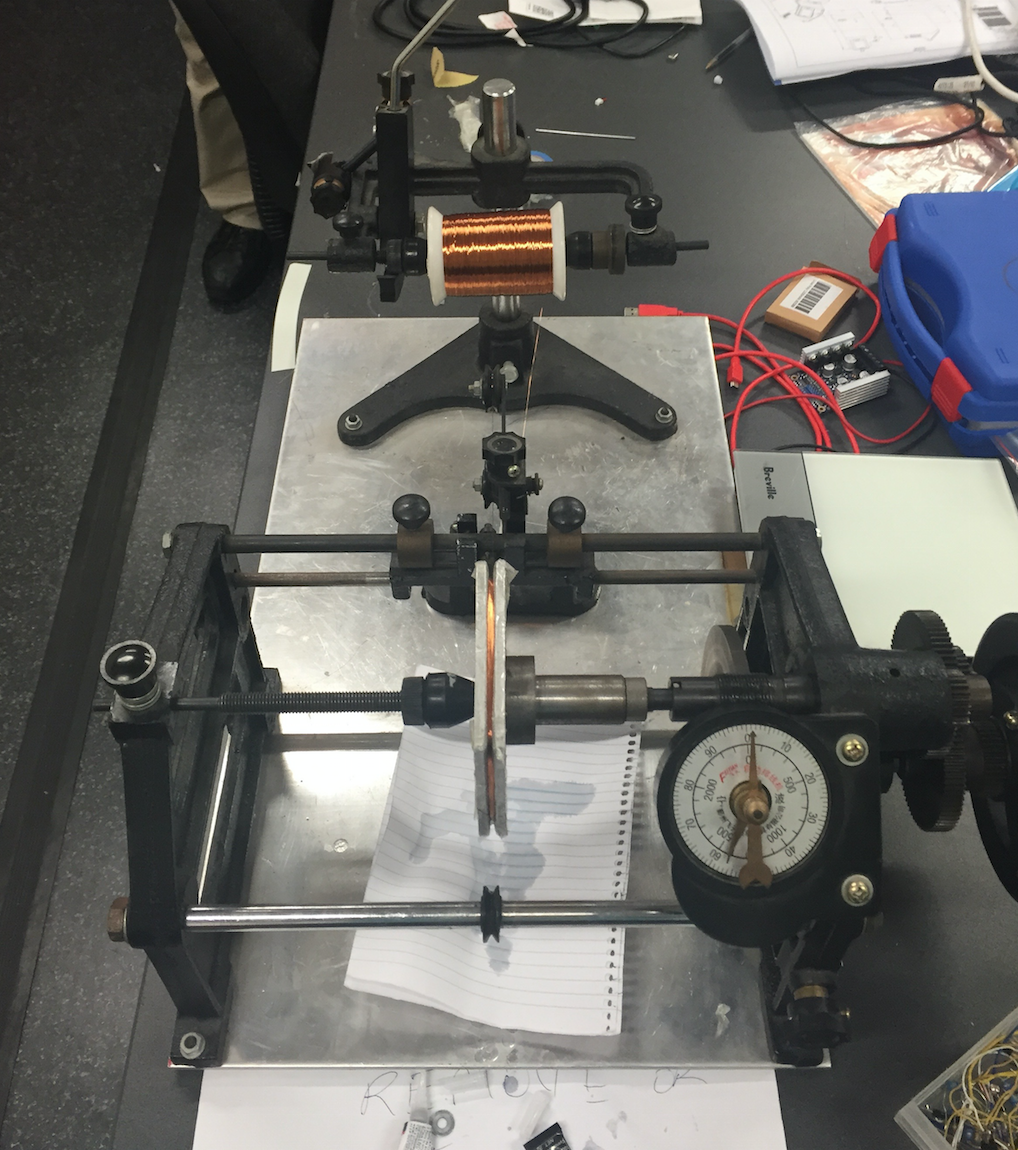
\includegraphics[scale = 0.35]{./figures/Construction_2}
            \end{subfigure}
        \end{figure}
    \end{center}
    \vspace{-5mm}
    
    
    \item The wire at the very beginning of the coil was taped to the side of the mould to keep it separate from the coil so that it can be connected to the PCB.
    \item In order to measure the number of turns, the counter on the winder was set to zero.
    \item Twenty turns were completed and then a layer of super glue was added to the coiled wire on all four sides in order using a thin brush.
    \item Step 4 was repeated until the required number of turns was reached at which point another layer of glue was added to each side of the coil.
    \item The copper wire was cut and the wire at the very end of the coil was not stuck to the the main coil in order to provide a connection between the PCB and the magnetorquer.
    \item The glue was allowed to set for 10 mins and then the coil was carefully removed from the mould with the aid of the sticky tape.
    \item Once completed the ends of coil were carefully scraped with sandpaper in order to remove the protective coating and allow current to be passed through.
    \item The coil was testing by attaching it to a battery and using a compass to determine whether a magnetic field was being produced.
    \item An Ohmmeter was used to determine the resistance through the coil.  
\end{enumerate}
After testing both magnetorquers were found to have a slightly higher resistance than predicted with the first magnetorquer reading a resistance of 27.2$\Omega$ and the second magnetorquer reading 28.1$\Omega$.  This is roughly a 10\% increase on the predicted value of 24.9$\Omega$ and is most likely caused by the effect of the super glue which was not taken into consideration in the original calculations.  This will result in the magnetorquers using a slightly lower current as voltage is constant and have a lower maximum dipole value.  These values were calculated to be 0.138$Am^2$ and 0.137$Am^2$ for magnetorquers 1 and 2 respectively.  The image below depicts magnetorquer 1 just after construction.
\vspace{-6mm}
\begin{center}
    \begin{figure}[H]
        \caption{Completed Magnetorquer}
        \vspace{-4mm}
        \centering
        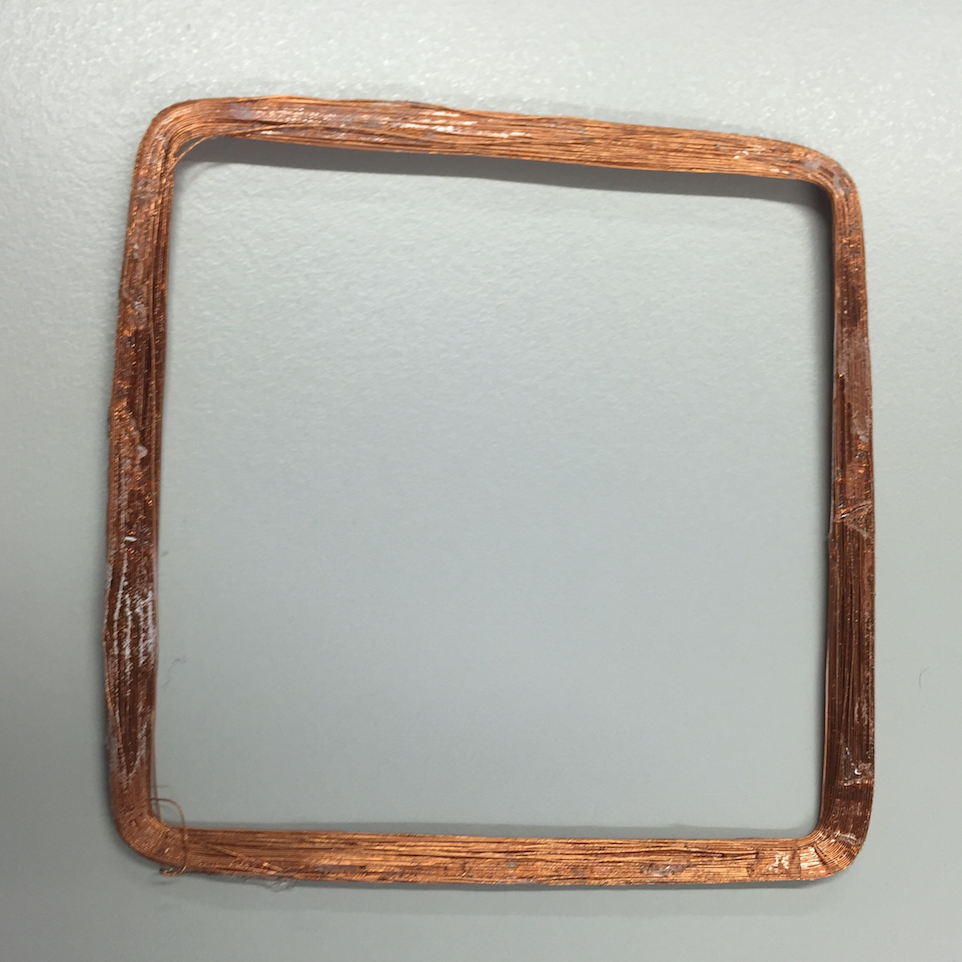
\includegraphics[scale = 0.4]{./figures/Magnetorquer}
    \end{figure}
\end{center}
\vspace{-5mm}
The magnetorquer is currently designated as TRL 4 based on the NASA scale.  It has been demonstrated to work in laboratory testing environment using coils of wire to model a magnetic field approximately ten times greater than that of the the earth's. However the component has not yet been fully integrated with the ACS system or been tested in the space environment.  

\subsection{Control System}
\subsubsection{Detumble Phase}
The first phase of the attitude control system will be the detumble phase in the period immediately after SnapSat's launch from the spacecraft.  The aim of the detumble phase is to reduce the rotation of the satellite to a near zero state.  There is no required attitude, that is  initialised in the second phase. Due to the high initial expected rate of tumble of 10 degrees per second, the photodiode sun sensor system will not be used in this phase.  Instead data from the IMU, primarily the gyro and the magnetorquer, will be utilised to determine the pitch, roll and yaw velocities.  Since, the IMU will be calibrated prior to launch it is expected that it will be most accurate during this initial phase.  The system will input the gyro and magnetometer IMU data into a B-Dot Controller. The B-Dot Controller will then calculate a torque in the opposing direction that matches the rate of change of the magnetic field and output the required PWM voltage to the magnetorquers.\\
\begin{center}
    $\dot{B} = \omega(t) \times B(t)$\\
    $m(t) = -k \cdot \dot{B}(t)$\\
    $T_c(t) = m(t) \times B(t)$
\end{center}
\subsubsection{Attitude Control Phase}
After the angular velocity of the satellite decreases to a near zero value, the SnapSat will enter into the attitude control phase.  This will be the long term state of the satellite and it will allow the satellite to be controlled accurately enough to fulfill the operational design and take photographs of designated cities.  The control phase will take inputs from the accelerometer and photodiode sun sensor system and use them to determine the attitude of the satellite.  After defining a desired attitude for the SnapSate a PID function will be used to convert the error angle into a PWM voltage used to control the magnetorquers and drive the satellite towards the desired set point.\\
Raw sensor measurements can only give a rough estimation of state, so use of filtering is required for real time state estimation with minimal errors. Filtering is a method of determining the current state of the satellite based on current and past observations \cite{Kalman}.  The extended Kalman filter will be implemented in order to handle the non-linear  dynamics involved in spacecraft attitude estimation.  The extended Kalman filter "predicts the new state estimate based on previous data and then updates the result with the new observations" \cite{Kalman}.  Below is a diagram of the method by which the Kalman filter is implemented:\\
\vspace{-6mm}
\begin{center}`
    \begin{figure}[H]
        \caption{Model of Kalman Filter \cite{Kalman}}
        \vspace{-4mm}
        \centering
        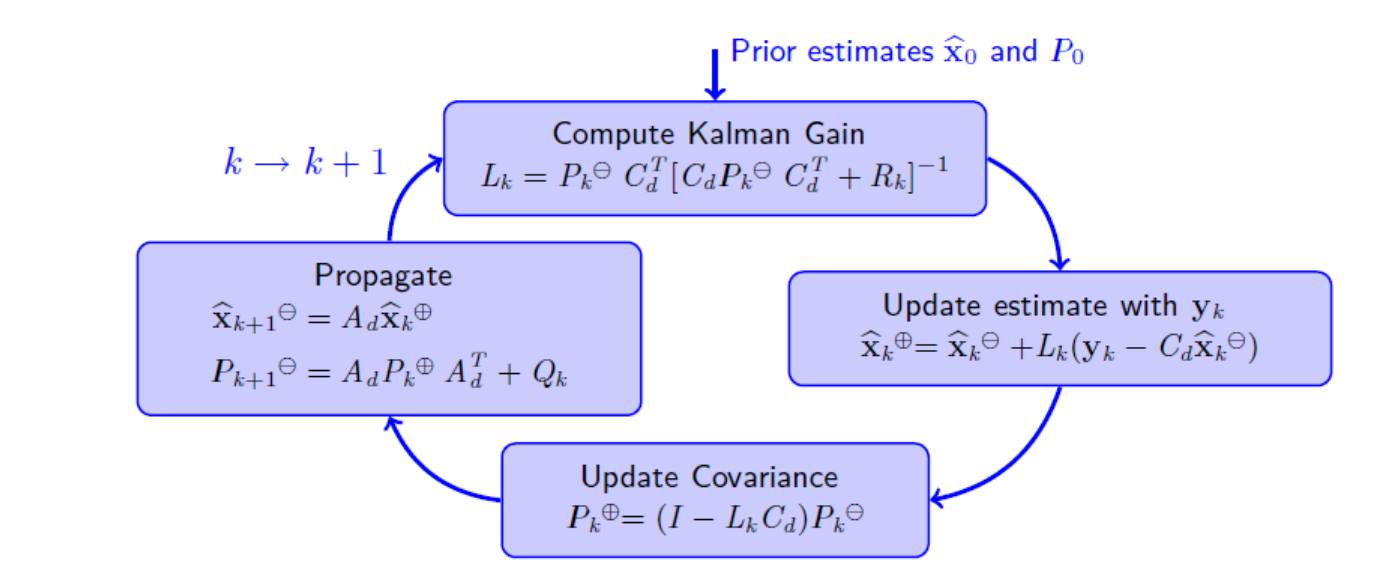
\includegraphics[width=\linewidth]{./figures/Kalman_Model}
    \end{figure}
\end{center}
\vspace{-5mm}
\subsubsection{Single Axis Control Model}
The dynamic model for the magnetorquer control system was produced by three fundamental equations:
\begin{center}
    $T = N \cdot I \cdot A \cdot B \cdot sin(\theta)$ \vspace{2mm} \\
    $V = I \cdot R$\vspace{2mm}\\
    $T = J \cdot \ddot{\theta}$\\
\end{center}
By combining these three equations and using a Laplace transform the following dynamic model was determined:
\begin{center}
    $\frac{\theta(s)}{V(s)} = \frac{N \cdot A \cdot B}{J \cdot R \cdot s^2 (s^2 + 1)}$
\end{center}
Thus using this function the following Simulink model was produced to determine the expected response of the satellite given certain inputs.
\vspace{-6mm}
\begin{center}`
    \begin{figure}[H]
        \caption{Simulink Model of Yaw Axis Control System}
        \vspace{-4mm}
        \centering
        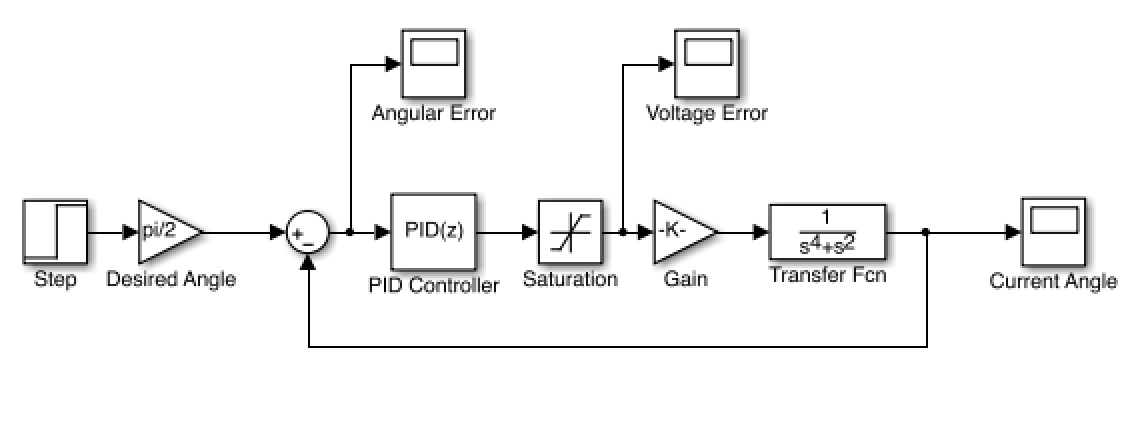
\includegraphics[scale = 0.8]{./figures/Simulink_ADCS_Model}
    \end{figure}
\end{center}
\vspace{-5mm}
Using this Simulink model for a yaw input of 90\textdegree (1.57rad) the response of the satellite was plotted.  As can be seen in the plot below, the system has a rise time of approximately 55 seconds while settling time is around 110 seconds.  Whilst there is no steady state error in the plot the angle continues to oscillate slightly in steady state.
\vspace{-6mm}
\begin{center}`
    \begin{figure}[H]
        \caption{Yaw Angle Rotation to 90\textdegree} 
        \vspace{-4mm}
        \centering
        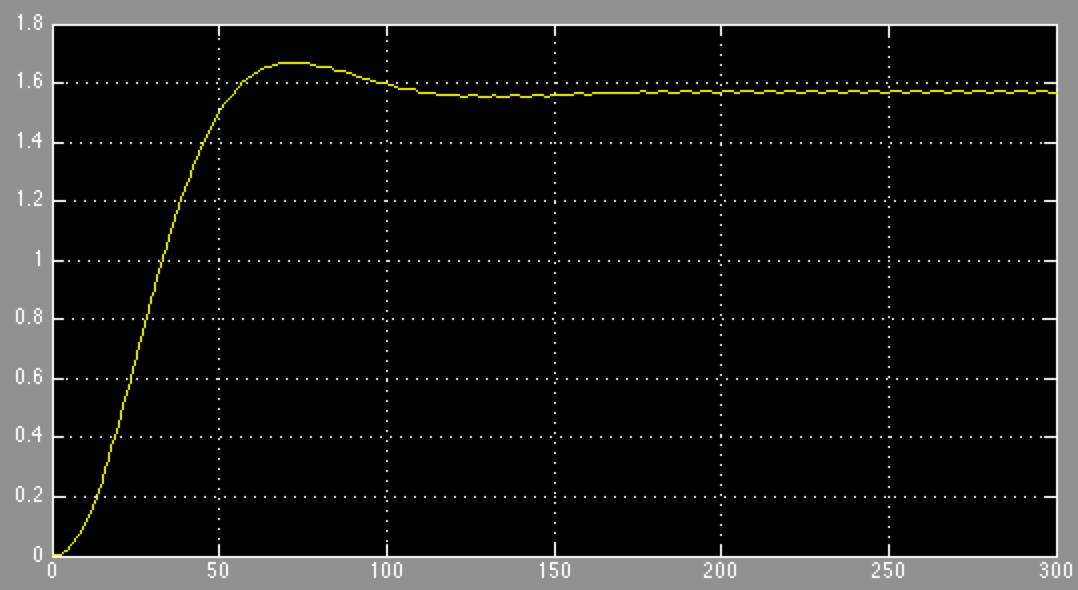
\includegraphics[width=\linewidth]{./figures/Yaw_Angle}
    \end{figure}
\end{center}
\vspace{-5mm}
\subsection{Disturbance Torques}
When in orbit there are a number of environmental forces that will result in disturbance torques and affect the attitude of SnapSat over the course of its orbit.  Although these torques are minute when compared to torques experienced on earth, in space they can have a noticeable affect.\\
Magnetic disturbance torque is a result of the interaction between the residual dipole of the on-board electronic components and the earth's magnetic field.  The measured residual dipole moment of cubesats of similar size is around 0.01$Am^2$ \cite{Miller}.  The torque is given by the equation:
\begin{center}
    $T_{res} = M_{res} \cdot B_{Earth}$
\end{center} 
There will also be a torque on the satellite as a result of the the gravity gradient, which is a function of the principle moment of inertia and the angular rate of orbit.
\begin{center}
    $T_g = (I_{max} - I_{min}) \cdot 3 {n_{max}}^2$
\end{center}
Due to the fact that this is a low earth orbit at an altitude of 350km there is atmospheric drag force on the satellite given by the following equation:
\begin{center}
    $F_d = \frac{1}{2} \rho v^2 C_d A (N \cdot D)$
\end{center}
This drag force results in an atmospheric drag torque which is calculated by multiplying the force by the distance between the centre of aerodynamic pressure and the geometric centre which is known as the lever arm and denoted by P.   
\begin{center}
    $T_d = P \times F_d$
\end{center}
Finally solar radiation pressure also implements a torque on the satellite given by the equation:
\begin{center}
    $T_S = \frac{\phi}{c^2} A (1 + Q)(N\cdot S)d$
\end{center}
Using these equations the max disturbance torques for SnapSat in orbit were estimated based on a mixture of data from SnapSat itself and other comparable satellites currently in orbit. 
\begin{table}[H]
    \begin{center}
        \caption{Estimated Disturbance Torques on SnapSat}
        \begin{tabular}{|c|c|}
            \hline
            Torque Type & $N \cdot m$ \\
            \hline
            Residual Dipole Torque & $3.4 \times 10^{-7}$ \\
            \hline
            Aerodynamic Torque & $1.8 \times 10^{-7}$ \\
            \hline
            Gravity Gradient Torque & $2.48 \times 10^{-9}$ \\
            \hline
            Solar Pressure Torque & $9.86 \times 10^{-10}$ \\
            \hline
            Total Disturbance Torque & $5.23 \times 10^{-7}$ \\
            \hline
        \end{tabular}
    \end{center}
    \vspace{-6mm}
\end{table}
As can be seen from the table, for an altitude of 350km the two largest disturbance torques are residual dipole and aerodynamic torque.